\begin{figure}[t]
\centering
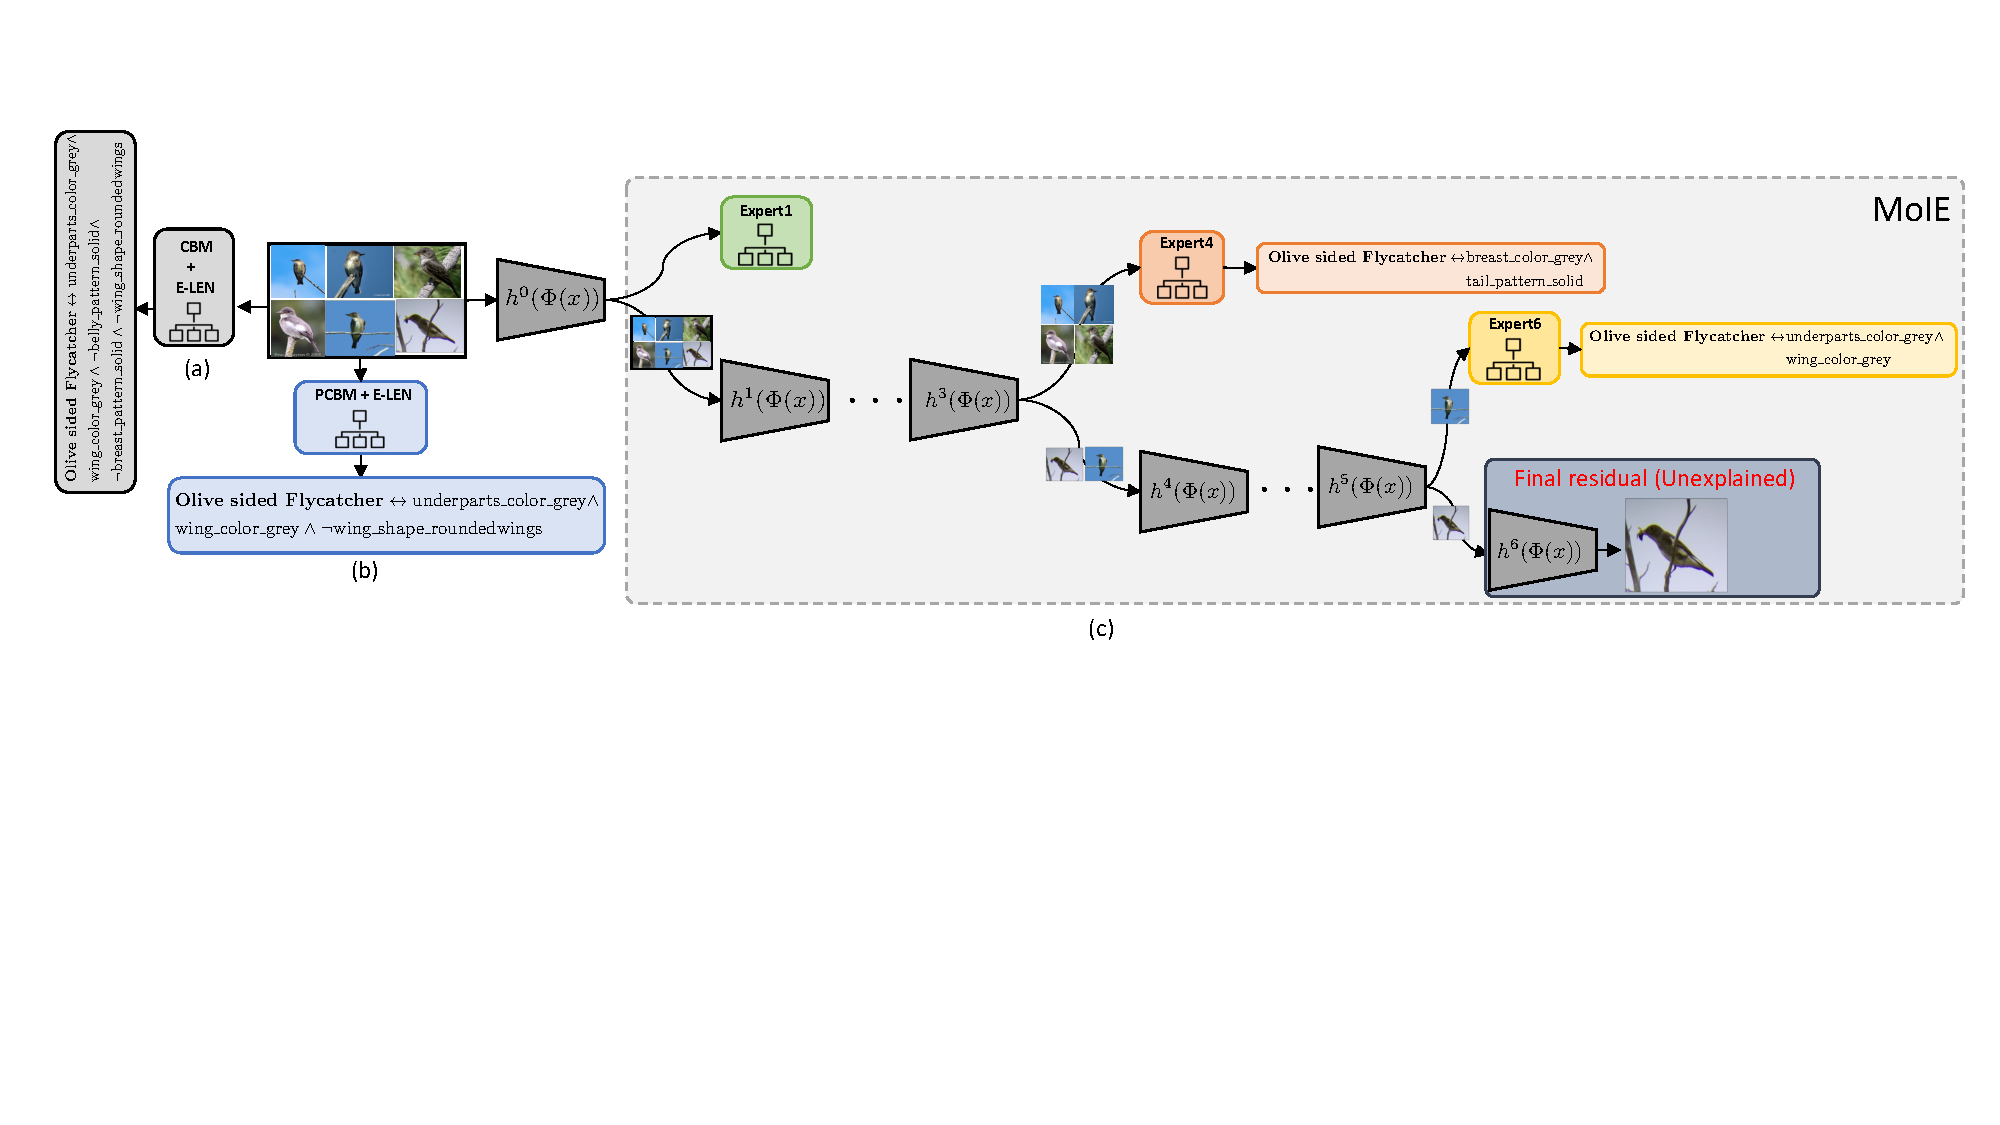
\includegraphics[width=1 \linewidth]{figures/Supp/Olive_sided.pdf}
\vspace{-10pt}
\caption{Construction logical explanations of the samples of a category, ``Olive sided Flycatcher'' in the CUB-200 dataset for (a) VIT-based sequential CBM + E-LEN as an \emph{interpretable by design} baseline, (b) VIT-based PCBM + E-LEN as a posthoc based baseline, (c) various experts in MoIE at inference. This is an example where the final residual covers the unexplained sample, which is ``harder'' to explain (indicated in \emph{red}). Also, MoIE can capture more instance-specific concepts than generic ones by the baselines.}
\label{fig:local_ex_cub_olive_sided}
\vspace{-2.5pt}
\end{figure}


\begin{figure}[h]
\centering
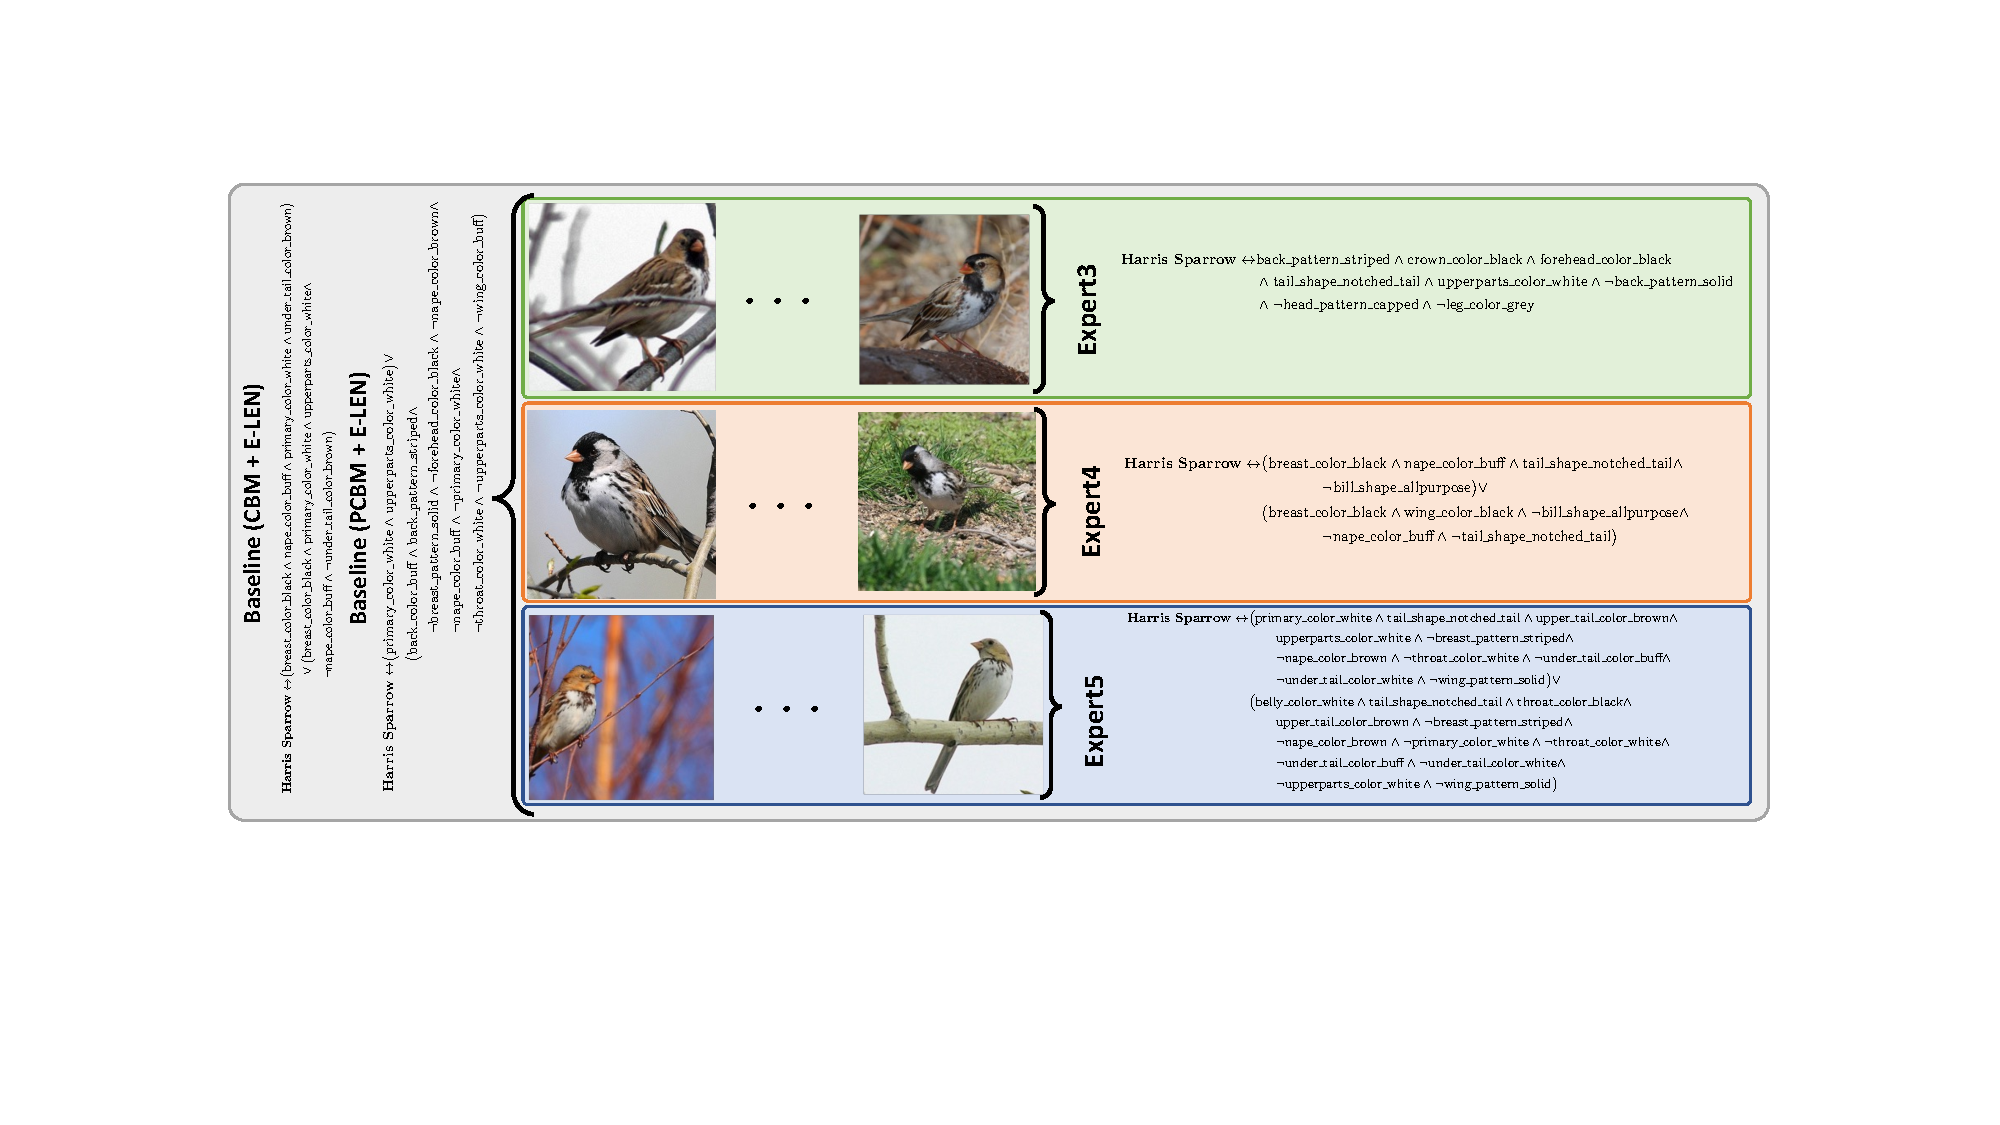
\includegraphics[width=1 \linewidth]{figures/Supp/Harris_sparrow.pdf}
\vspace{-10pt}
\caption{Construction logical explanations of the samples of a category, ``Harris Sparrow'' in the CUB-200 dataset for (a) VIT-based sequential CBM + E-LEN as an \emph{interpretable by design} baseline, (b) VIT-based PCBM + E-LEN as a posthoc based baseline, (c) various experts in MoIE at inference.}
\label{fig:local_ex_cub_harris}
\vspace{-2.5pt}
\end{figure}

\begin{figure}[h]
\centering
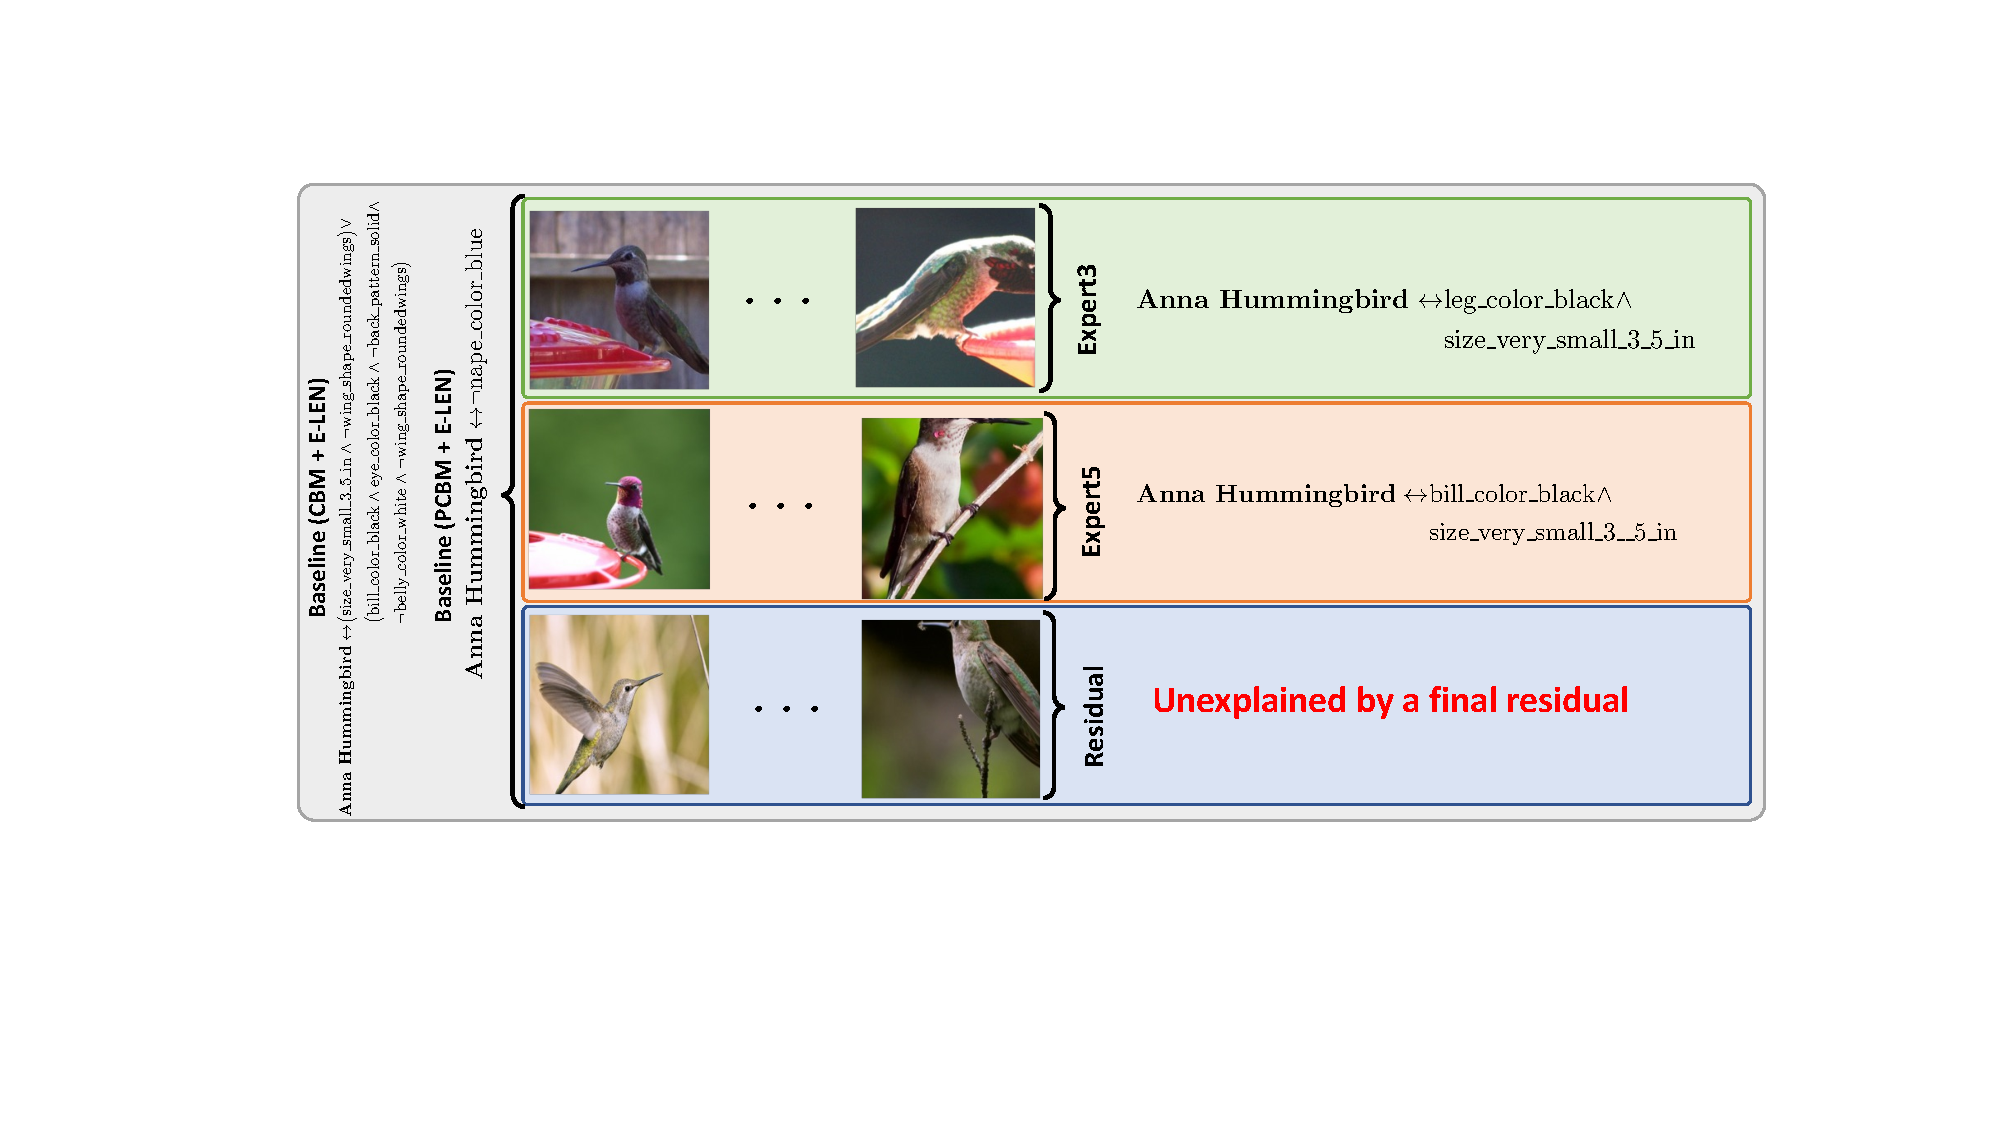
\includegraphics[width=1 \linewidth]{figures/Supp/Anna_hummingbird.pdf}
\vspace{-10pt}
\caption{Construction logical explanations of the samples of a category, ``Anna Hummingbird'' in the CUB-200 dataset for (a) VIT-based sequential CBM + E-LEN as an \emph{interpretable by design} baseline, (b) VIT-based PCBM + E-LEN as a posthoc based baseline, (c) various experts in MoIE at inference.}
\label{fig:local_ex_anna}
\vspace{-2.5pt}
\end{figure}

\begin{figure}[h]
\centering
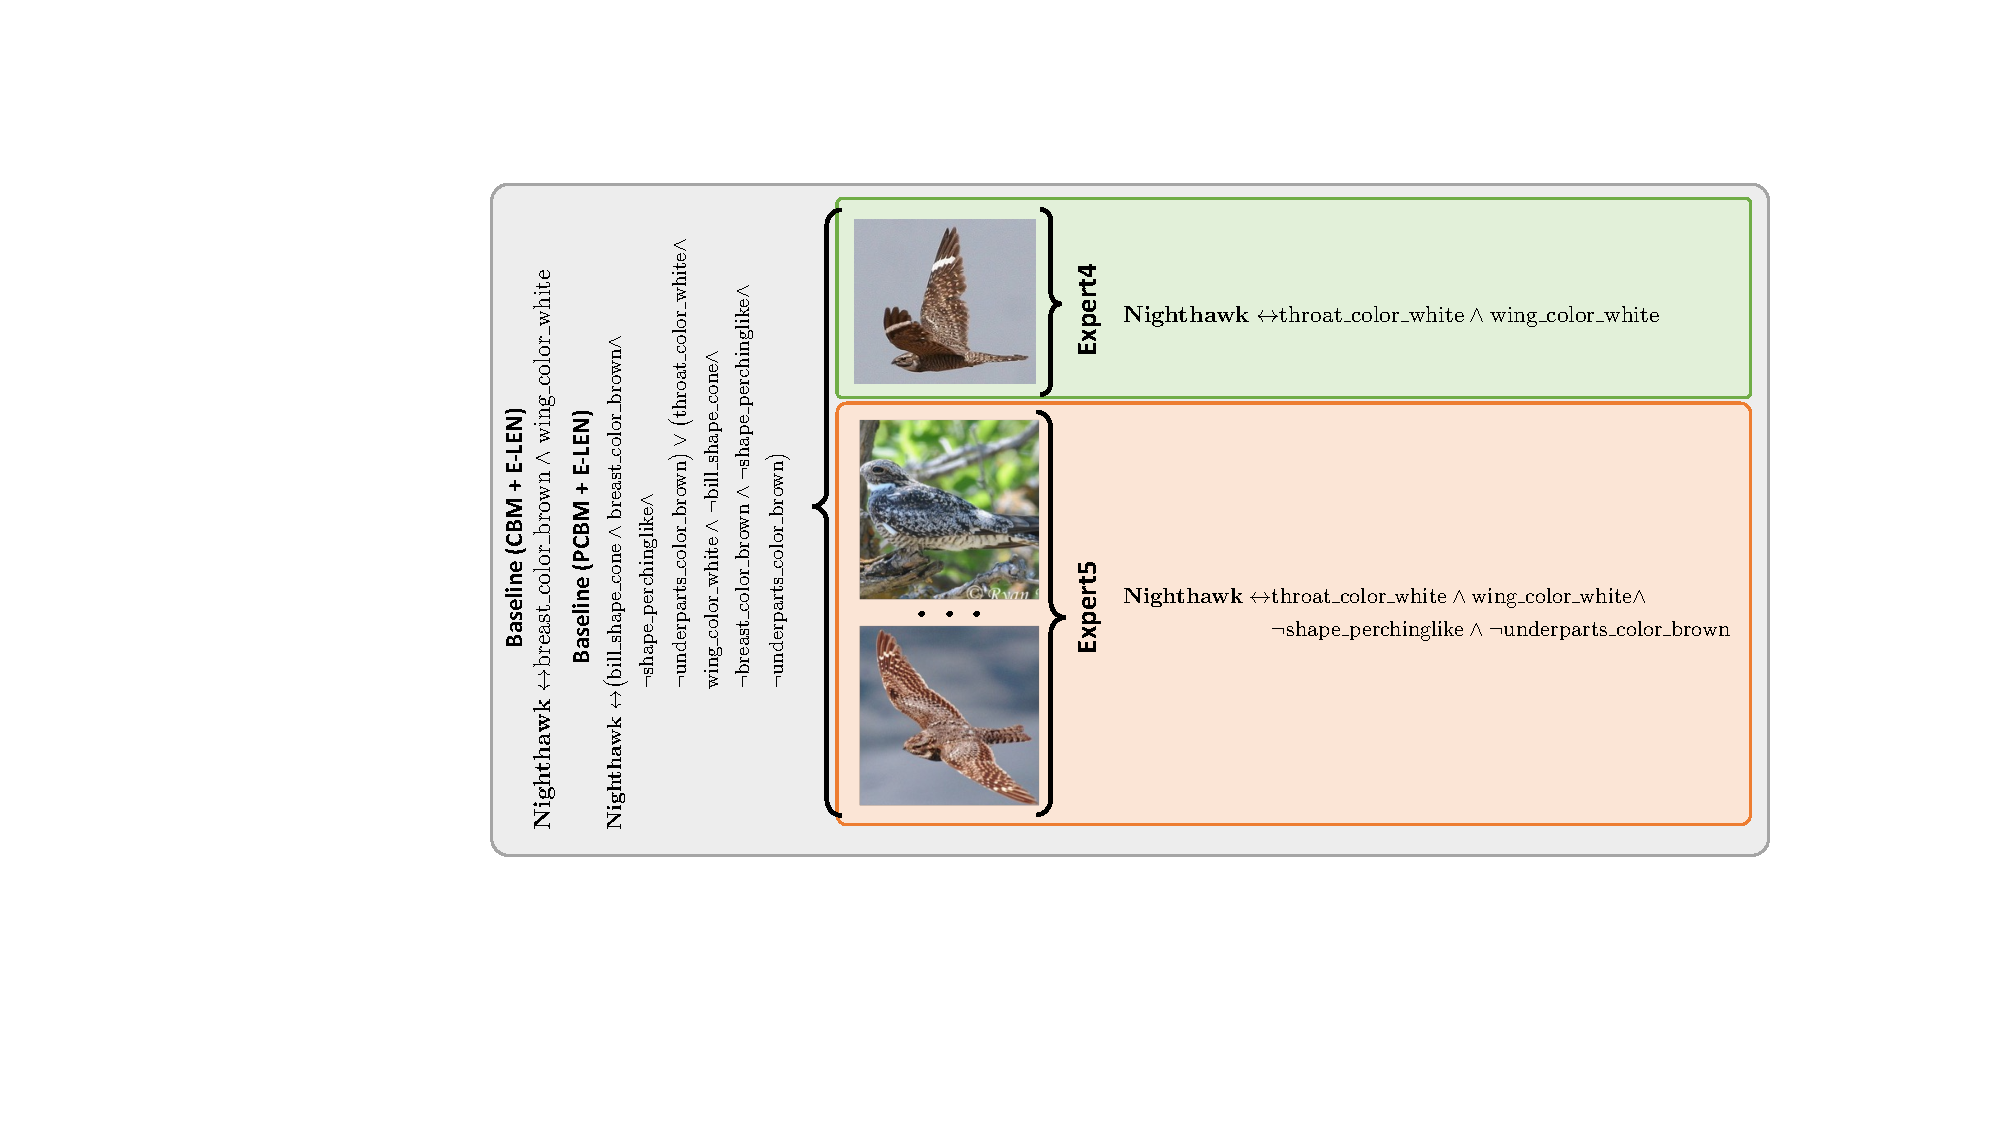
\includegraphics[width=1 \linewidth]{figures/Supp/Nighthawk.pdf}
\vspace{-10pt}
\caption{Construction logical explanations of the samples of a category, ``Nighthawk'' in the CUB-200 dataset for (a) VIT-based sequential CBM + E-LEN as an \emph{interpretable by design} baseline, (b) VIT-based PCBM + E-LEN as a posthoc based baseline, (c) various experts in MoIE at inference. }
\label{fig:local_ex_nighthawk}
\vspace{-2.5pt}
\end{figure}

\begin{figure}[h]
\centering
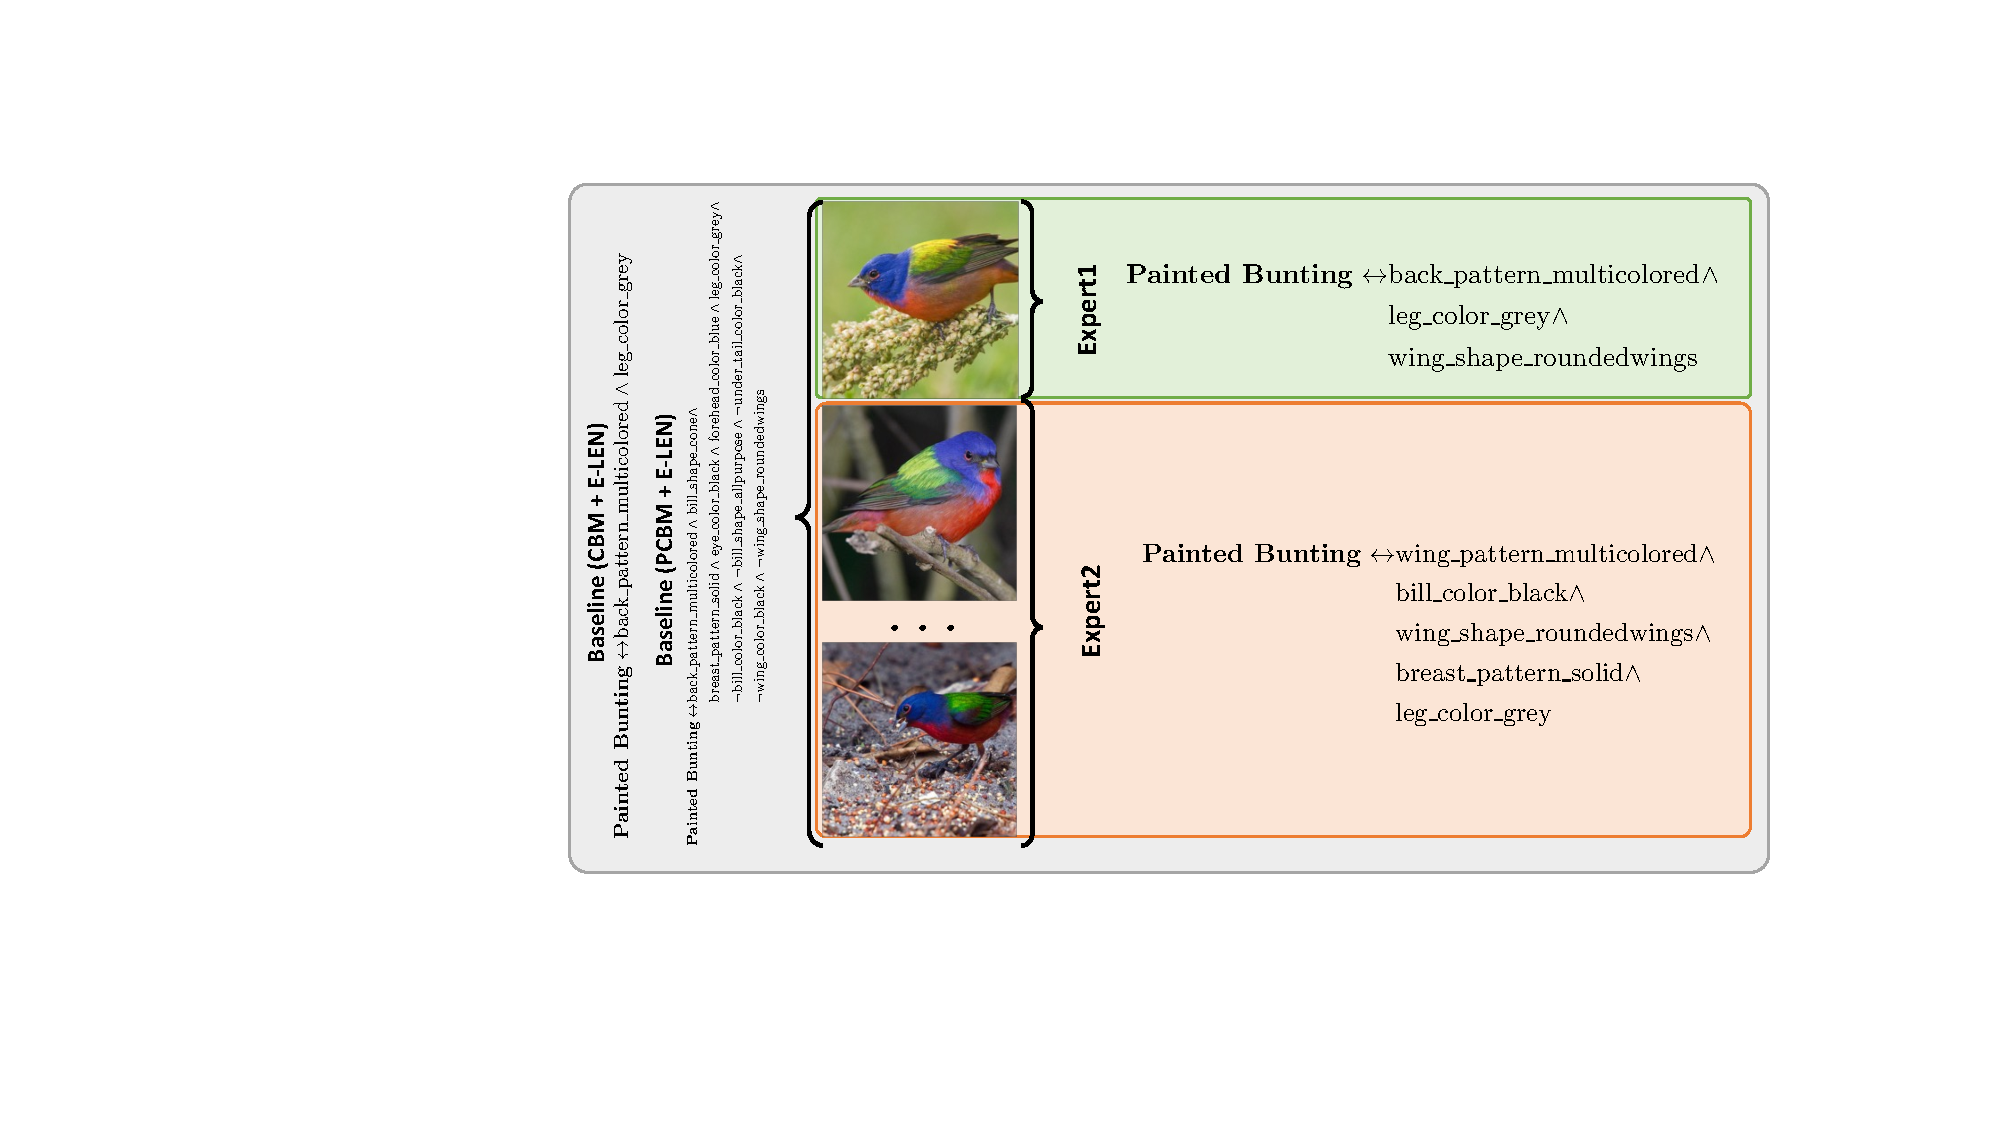
\includegraphics[width=1 \linewidth]{figures/Supp/Painted_bunting.pdf}
\vspace{-10pt}
\caption{Construction logical explanations of the samples of a category, ``Painted Bunting'' in the CUB-200 dataset for (a) VIT-based sequential CBM + E-LEN as an \emph{interpretable by design} baseline, (b) VIT-based PCBM + E-LEN as a posthoc based baseline, (c) various experts in MoIE at inference. }
\label{fig:local_ex_cub_painted}
\vspace{-2.5pt}
\end{figure}

\cref{fig:local_ex_cub_olive_sided} shows the construction of instance-specific local FOL explanations of a category, ``Olive sided Flycatcher'' in the CUB-200 dataset for the VIT-based baselines and MoIE. In this example, the final expert6 covers the relatively ``harder'' sample.~\cref{fig:local_ex_cub_harris},~\cref{fig:local_ex_anna},~\cref{fig:local_ex_nighthawk},~\cref{fig:local_ex_cub_painted} shows more such FOL explanations. All these examples demonstrate MoIE's high capability to identify more meaningful instance-specific concepts in FOL explanations. In contrast, the baselines identify the generic concepts for all samples in a class.



